% !TeX encoding = UTF-8
% !TeX program = pdfLaTeX
% !TeX root = matlab-exercises-emaip.tex
% !TeX spellcheck = en_GB
\section{Control structures}

\begin{wrapfigure}{r}[1cm]{4cm}
\centering
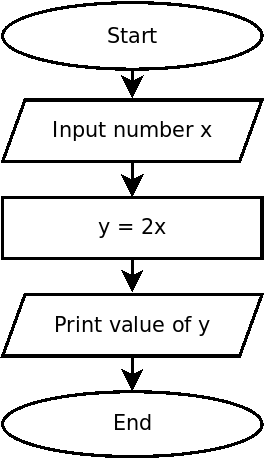
\includegraphics[width=3cm]{pic/flowchart_linear_program_flow.png}
\caption{Linear program flow.}
\label{figLinearProgramFlow}
\end{wrapfigure}
Until now, we have only looked at programs that progress linearly through a set of 
operations / commands to Matlab.
Such a linear program flow is shown here in figure \ref{figLinearProgramFlow}.
To read the flow chart, locate the round bubble with the 
text \emph{start} and then follow the arrows from element to 
element.
A matlab script that has the same structure as the flowchart is shown here:
\begin{lstlisting}
x = input('Enter a number: ');
y = 2*x;
fprintf("Twice the input value is %d\n", y);
\end{lstlisting}



In this chapter methods for controlling the flow of execution of programs will be 
discussed.
In the flow chart this will be seen as branches, where the program flow at certain 
locations can choose between two or more branches. 
This is depicted with a diamond shape (a square rotated 45 degrees).
In some cases the branches will merge together after some time.
In some cases one of the branches will go back to an earlier visited state in the program.

Such branches in the program logic, allows us to write more complicated programs.


\subsection{If statements}

The first structure to learn for controlling the program flow 
is the \emph{if} structure.
The structure lets the programmer choose which one of two paths the 
program execution will follow.
\begin{lstlisting}
x = input('Enter a number: ');
if( mod(x, 2) == 0)
    fprintf("The number is even!\n");
else
    fprintf("The number is odd!\n");
end\end{lstlisting}
In the code above, \verb!mod(x, 2) == 0! checks whether the number $x$ 
is even. If $x$ is even, the expression is true and the first branch will be 
executed.  If the expression is false, the \verb!else! branch will be executed.
This is visualized in figure \ref{figFlowchartWithIfBranch}.
The condition (\verb!mod(x, 2) == 0!) decides which path of the two branches will be followed.
The condition should be a boolean value, that is either true or false.
In a number different from zeros is inserted it is recognized as a true value.

\begin{figure}
\centering
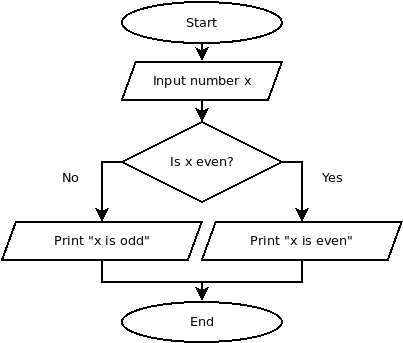
\includegraphics[width=6cm]{pic/flowchart_simple_branch.png}
\caption{Flowchart with if branch.}
\label{figFlowchartWithIfBranch}
\end{figure}



%\todo[inline]{Use this as inspiration for introducing if statements \url{https://www.learnbyexample.org/python-if-else-elif-statement/}¨}

%\todo[inline]{Experiment with decision tables for specifying branching behaviour \url{https://www.hillelwayne.com/decision-tables/}}




\subsection{For loops}

\begin{figure}
\centering
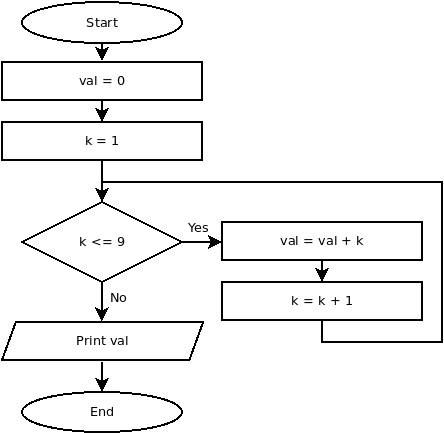
\includegraphics[width=8cm]{pic/flowchart_for_loop.png}
\caption{Flowchart with a for loop.}
\label{figFlowchartWithAForLoop}
\end{figure}
Consider the task of adding all integers from 1 to 9
and storing the result in the variable \verb!val!;  
this can be achieved with the following code 
\begin{lstlisting}
val = 1 + 2 + 3 + 4 + 5 + 6 + 7 + 8 + 9
\end{lstlisting}
This is straightforward to write, but does not scale
as well as possible.
Adding all integers from 1 to 100 with a similar method
is still possible although impractical.
The task of adding all integers from 1 to 1000000 
is impractical, so lets look at better ways of doing such 
calculations.

The first step to make the code easier to write, does the
direct opposite thing; it makes the code much longer, but it 
also gives it a more repeating structure, which soon will be 
exploited 
\begin{lstlisting}
val = 0;
val = val + 1;
val = val + 2;
val = val + 3;
val = val + 4;
val = val + 5;
val = val + 6;
val = val + 7;
val = val + 8;
val = val + 9;
val
\end{lstlisting}
It still bothers me that the line where \verb!val! is updated
changes from line to line.
To avoid this a helper variable $k$ is introduced.
Before each update of \verb!val! the value of $k$ is 
increased by one and then the update rule can be used.
\begin{lstlisting}
val = 0;
k = 1;
val = val + k;
k = 2;
val = val + k;
k = 3;
val = val + k;
k = 4;
val = val + k;
k = 5;
val = val + k;
k = 6;
val = val + k;
k = 7;
val = val + k;
k = 8;
val = val + k;
k = 9;
val = val + k;
val
\end{lstlisting}
To tell matlab to repeat the update rule \verb!val = val + k! for
all values of $k$ from 1 to 9, the following code can be used:
\begin{lstlisting}
val = 0;
for k = 1:9
    val = val + k;
end
val
\end{lstlisting}
Compared with the first approach of manually typing
all the integers in the range 1 to 9, it takes a bit more space, 
but the code has become much easier to adapt to other problems.


\begin{ex}\label{exSumIntegersUp100}%
Determine the value of 
\begin{align*}
\sum_{k = 1}^{100} k = 1 + 2 + 3 + \ldots + 98 + 99 + 100
\end{align*}
In other words calculate the sum of all integers from 1 to 100.
\begin{hint}
A for loop will be a good structure to use.
The answer is 5050.
\end{hint}
\begin{sol}
A solution is:
\begin{lstlisting}
val = 0;
for k = 1:100
    val = val + k;
end
val
\end{lstlisting}
\end{sol}
\end{ex}

\begin{ex}
Determine the value of 
\begin{align*}
\sum_{k = 1}^{100} \sin(k) = \sin(1) + \sin(2) + \ldots + \sin(99) + \sin(100)
\end{align*}
\begin{hint}
A for loop will be a good structure to use.
The answer is -0.1272.
\end{hint}
\begin{sol}
A solution is:
\begin{lstlisting}
val = 0;
for k = 1:100
    val = val + sin(k);
end
val
\end{lstlisting}
\end{sol}
\end{ex}


\begin{ex}
Test the following expression by selecting a positive integer $n$
and evaluate both sides of the expression using the selected value.
\begin{align*}
\sum_{i = 1}^n i = \frac{n \cdot (n + 1)}{2}
\end{align*}
Repeat this with three different value of $n$.
\begin{hint}
Look at the code from exercise \ref{exSumIntegersUp100}.
It can be adapted to evaluate the left hand side of the expression.
\end{hint}
\begin{sol}
A solution is:
\begin{lstlisting}
n = 234;
val_left = 0;
for k = 1:n
    val_left = val_left + k;
end
val_left
val_right = n * (n + 1) / 2
\end{lstlisting}
\end{sol}
\end{ex}


\begin{ex}
Test the following expression by selecting a positive value $a$
which is not one and an integer $n$
and evaluate both sides of the expression using the selected value.
\begin{align*}
\sum_{i = 0}^n a^i = \frac{1 - a^{n + 1}}{1 - a}
\end{align*}
Repeat this with three different value of $n$.
\begin{hint}
Look at the code from exercise \ref{exSumIntegersUp100}.
It can be adapted to evaluate the left hand side of the expression.
\end{hint}
\begin{sol}
A solution is:
\begin{lstlisting}
a = 1.2;
n = 43;
val_left = 0;
for k = 0:n
    val_left = val_left + a^k;
end
val_left
val_right = (1 - a^(n + 1)) / (1 - a)
\end{lstlisting}
\end{sol}
\end{ex}




\subsection{Formatting variables with sprintf}

To show a numeric value in a string in a specific way can be 
done with the function \verb!sprintf!.
The command takes one or more input arguments.
The first argument is a format specifier and the rest
of the arguments are the values that will be inserted 
into the string.
Eg. to display the value of $\pi$ with 5 decimals
along with a descriptive text, the following code 
can be used:
\begin{lstlisting}
>> sprintf("The value of pi is: %.5f", pi)
ans = "The value of pi is: 3.14159"
\end{lstlisting}
It is also possible to insert multiple variables
of different types into the string, this is demonstrated 
here.
\begin{lstlisting}
>> sprintf("My name is %s. I was born in %d.", "Henrik", 1983)
ans = "My name is Henrik. I was born in 1983."
\end{lstlisting}
To display the formatted string in the console
instead of returning it, the function
\verb!fprintf! can be used.
\begin{lstlisting}
>> fprintf("Pi is %.2f\n", pi)
Pi is 3.14
\end{lstlisting}
Read more about the format specifiers in the documentation
\begin{lstlisting}
>> help sprintf
\end{lstlisting}




\begin{ex}
Create a function for entering phasors into matlab.
The function signature should be:
\begin{lstlisting}
function res = phasor(magnitude, direction)
\end{lstlisting}
where \verb!magnitude! is the amplitude of the 
phasor to generate and \verb!direction! is the phase offset
in degrees.
Use the following examples to test the function:
\begin{lstlisting}
>> phasor(2, 45)
ans = 1.4142 + 1.4142i
>> phasor(3, 90)
ans = 0.0000 + 3.0000i
>> phasor(1, 135)
ans = -0.7071 + 0.7071i
\end{lstlisting}
\begin{hint}
A phasor is defined as 
\begin{align*}
\textrm{magnitude} \cdot e^{i \cdot \textrm{direction}}
\end{align*}
where the direction is specified in radians
\end{hint}
\begin{sol}
A solution is:
\begin{lstlisting}
function res = phasor(magnitude, direction)

res = magnitude * exp(1i*direction*pi / 180);

end\end{lstlisting}
\end{sol}
\begin{solutionfile}{phasor_test.m}
function tests = phasor_test
    tests = functiontests(localfunctions);
end


%% Format phasor for human reading
function test01(testCase)
    actual_value = phasor(2, 45);
    expected_value = 2*sin(pi / 4) + 2*cos(pi/4)*1i;
    testCase.verifyEqual(actual_value, expected_value,...
        'RelTol', 0.000001);
end
\end{solutionfile}
\begin{solutionfile}{phasor.m}
function res = phasor(magnitude, direction)

res = magnitude * exp(1i*direction*pi / 180);

end
\end{solutionfile}
\end{ex}


\begin{ex}
Create a function that displays the magnitude and 
phase offset (in degrees) of a phasor.
Both magnitude and phase offset should be shown with six 
decimal values.
The function signature should be:
\begin{lstlisting}
function res = show_phasor(value)
\end{lstlisting}
Use the following examples to test the function:
\begin{lstlisting}
>> show_phasor(1+i)
ans = "1.414214 < 45.000000"
>> show_phasor(2-3*i)
ans = "3.605551 < -56.309932"
\end{lstlisting}
\begin{hint}
The functions \verb!abs! and \verb!angle! will be helpful together with the \verb!sprintf! function.
\end{hint}
\begin{sol}
A solution is:
\begin{lstlisting}
function res = show_phasor(value)

magnitude = abs(value);
phase_offset = angle(value) * 180 / pi;
res = sprintf("%.6f < %.6f", magnitude, phase_offset);

end
\end{lstlisting}
\end{sol}
\begin{solutionfile}{show_phasor.m}
function res = show_phasor(value)

magnitude = abs(value);
phase_offset = angle(value) * 180 / pi;
res = sprintf("%.6f < %.6f", magnitude, phase_offset);

end
\end{solutionfile}
\begin{solutionfile}{show_phasor_test.m}
function tests = show_phasor_test
    tests = functiontests(localfunctions);
end


%% Format phasor for human reading
function test01(testCase)
    actual_value = show_phasor(2);
    expected_value = "2.000000 < 0.000000";
    testCase.verifyEqual(actual_value, expected_value);
end

function test02(testCase)
    actual_value = show_phasor(2 + 2*1i);
    expected_value = "2.828427 < 45.000000";
    testCase.verifyEqual(actual_value, expected_value);
end
\end{solutionfile}
\end{ex}


